\section{Backend}

\subsection{Basics of system architecture}
\subsubsection{Data and logic separation}\label{DataLogic}
\begin{figure}[!h]
	\centering
	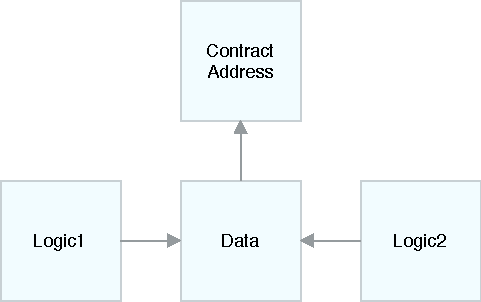
\includegraphics[width=0.65\textwidth]{img/DataLogic.pdf}
	\caption{Data-Logic pattern}
\end{figure}
Due to contract limited potential of upgrade and maintenance after the deployment on blockchain, contracts have been splitted in two different parts, each of ones is saved in the corresponding contract. This way one contract contains the data structure of an object and the other one contains the logical complex methods that refers to data.
This pattern allow the developer to update and deploy only the new logical contract, keeping the data contract persistent and not losing all the old data. \\
The part that structures the data contains only the data and the methods that let the user to retrieve (getters) or modify (setters) them. Not all the users of the blockchain should have the right to access the data: the contracts on the blockchain are accessible by everyone. To fix this problem, the majority of the methods contains in their header an access modifier that give access only to the authorized users. \\
The third element of this pattern is the ContractManager: this contract contains only the newest version of the contracts addresses. This is useful for two main reasons:
\begin{enumerate}
	\item Easier contract structure: it's ordinary that a data contract is used by multiple logic contracts like in the \hyperref[DataLogic]{example above}; in this case it has to save and set all the related logical contracts address needed for the modifiers. Instead, using the ContractManager, developer have to save only the ContractManager address, in the Data contract, that will include all the other contracts addresses;
	\item Second one is logically derived from the point above: if a logic contract is updated and re-deployed (and consequently has a new contract address), the developer should have had to manually set the new address in all the n-contracts that contain the old one. Using the ContractManager, instead, the developer have to set the new deployed contract address only in the ContractManager and all the n-contracts will be updated.
\end{enumerate}
Consequently this pattern make it easier for the developer to update the contracts and involves lower costs in the long term.
\newpage
\subsubsection{Contracts description}
There is only one instance of a contract. To obtain multiple instance of an object there are struct inside contracts, this way you can gather consistent data together. Mapping are used for saving reference to struct object and arrays to iterate on that reference: in Solidity you can't obtain the keys of a mapping, so you need to save that keys in the array.
There is a brief summary of the application's contracts:
\begin{itemize}
	\item \textbf{ContractManager}: like we said before, this contract contain all the addresses of the contracts and the address of the university;
	\item \textbf{UserData}: contains the application's users data, saved in a struct called User. This contract also contain the getter and setter methods for the data private fields;
	\item \textbf{UserLogic}: contains methods useful for not registered or not logged user. It uses UserData;
	\item \textbf{ExamData}: contains the university exams application data, saved in a struct called Exam. This contract also contain the getter and setter methods for the data private fields;
	\item \textbf{ClassData}: contains the university didactic activities application data, saved in a struct called Class. This contract also contain the getter and setter methods for the data  private fields. It uses ExamData;
	\item \textbf{DegreeData}: contains the university degree courses application data, saved in a struct called Degree. This contract also contain the getter and setter methods for the data private fields;
	\item \textbf{StudentData}: contains the university students' application mapping, used for simplify queries, considering that most users will be students. This contract also contain the getter and setter methods for the data mapping;
	\item \textbf{Student}: contains methods useful for students. It uses UserData, ExamData and StudentData;
	\item \textbf{Teacher}: contains methods useful for professors. It uses UserData and ExamData;
	\item \textbf{Admin}: contains methods useful for admins and university. It uses UserData, ExamData, DegreeData.
	
\end{itemize}

In the next section, you can find more details about the contracts above.

\subsection{UML Diagram}

\subsubsection{ContractManager}
\begin{figure}[!h]
	\centering
	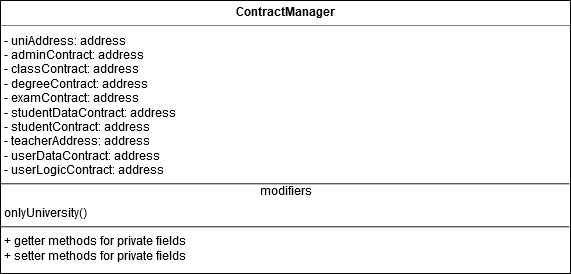
\includegraphics[width=0.65\textwidth]{img/Contracts/ContractManager.png}
	\caption{ContractManager Diagram}
\end{figure}
\clearpage
\subsubsection{UserData}
\begin{figure}[!h]
	\centering
	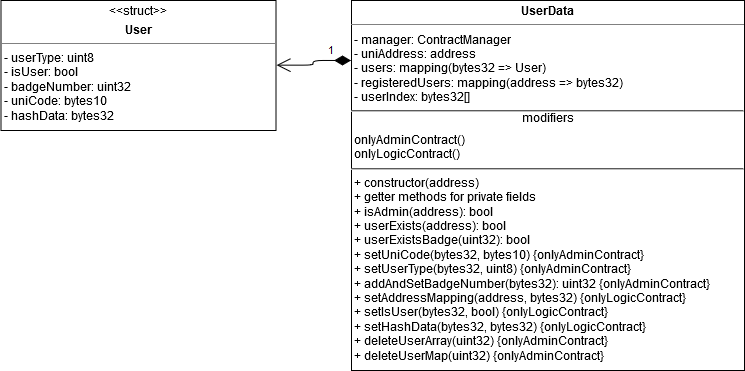
\includegraphics[width=0.65\textwidth]{img/Contracts/UserData.png}
	\caption{UserData Diagram}
\end{figure}
\subsubsection{UserLogic}
\begin{figure}[!h]
	\centering
	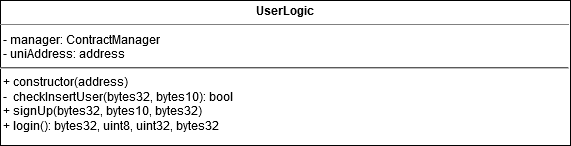
\includegraphics[width=0.65\textwidth]{img/Contracts/UserLogic.png}
	\caption{UserLogic Diagram}
\end{figure}
\subsubsection{Admin}
\begin{figure}[!h]
	\centering
	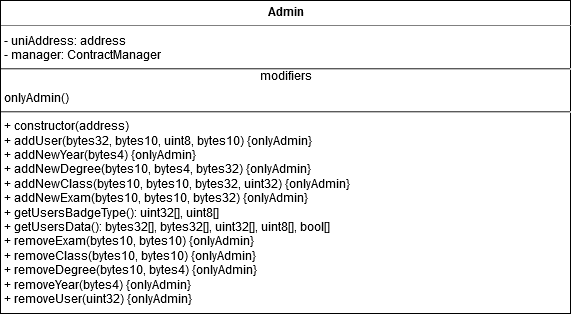
\includegraphics[width=0.65\textwidth]{img/Contracts/Admin.png}
	\caption{Admin Diagram}
\end{figure}
\clearpage
\subsubsection{Teacher}
\begin{figure}[!h]
	\centering
	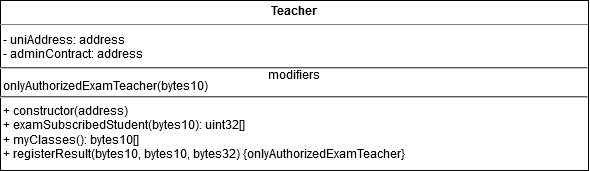
\includegraphics[width=0.65\textwidth]{img/Contracts/Teacher.png}
	\caption{Teacher Diagram}
\end{figure}
\subsubsection{StudentData}
\begin{figure}[!h]
	\centering
	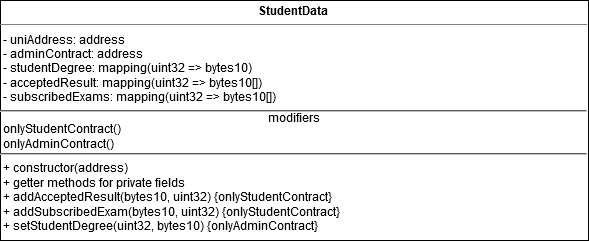
\includegraphics[width=0.65\textwidth]{img/Contracts/StudentData.png}
	\caption{StudentData Diagram}
\end{figure}

\subsubsection{Student}
\begin{figure}[!h]
	\centering
	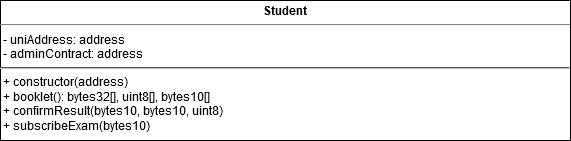
\includegraphics[width=0.65\textwidth]{img/Contracts/Student.png}
	\caption{Student Diagram}
\end{figure}
\clearpage
\subsubsection{DegreeData}
\begin{figure}[!h]
	\centering
	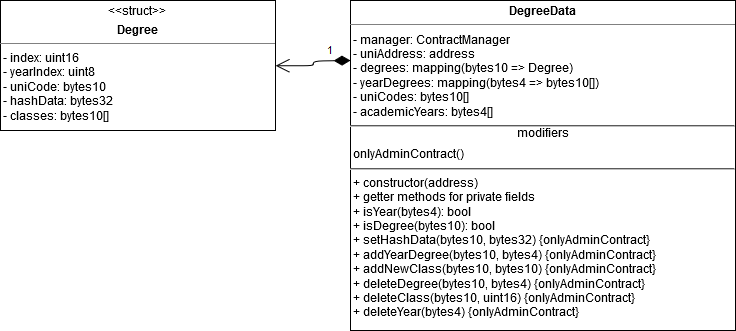
\includegraphics[width=0.65\textwidth]{img/Contracts/DegreeData.png}
	\caption{DegreeData Diagram}
\end{figure}
\subsubsection{ClassData}
\begin{figure}[!h]
	\centering
	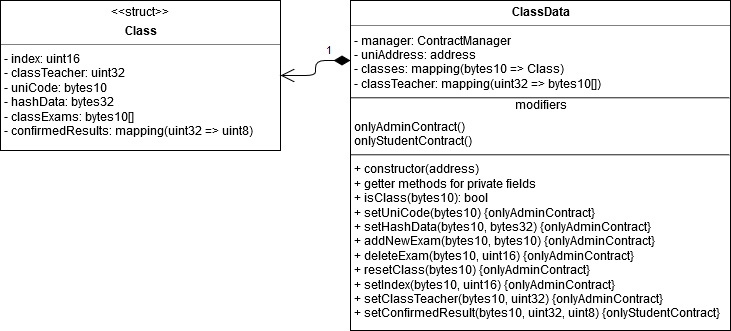
\includegraphics[width=0.65\textwidth]{img/Contracts/ClassData.png}
	\caption{ClassData Diagram}
\end{figure}
\subsubsection{ExamData}
\begin{figure}[!h]
	\centering
	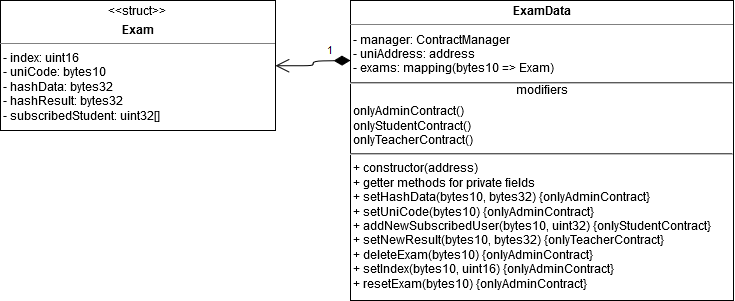
\includegraphics[width=0.65\textwidth]{img/Contracts/ExamData.png}
	\caption{ExamData Diagram}
\end{figure}
As you can see, like we said before, some contracts have a struct defined. This struct usually contain some common data: ad index for the array in the relative contract (in User we use badgeNumber like index), hashData that contain the hash for retrieve data from IPFS, uniCode for an indentifier of the object (note that for User struct it has a different meaning: it's just a code that the University give to you for the first authentication). All the other data in the struct is different between different contract. In the struct relative contract, there is the mapping for accessing the struct, together to other mapping and array of utilities.


\subsection{IPFS}
Saving data on the Ethereum blockchain is expensive and you can store only simple type data (like integer or string). To mitigate this problem external distributed database is used: we choose IPFS for it's easy of use and because it's in a pretty advanced version. 
For instructions on how to use IPFS you can see \hyperref[IPFS]{this} section. The developer should follow this guidelines to choose to save an information on blockchain or IPFS:
\begin{enumerate}
	\item Data used to query on contract should be saved on blockchain to prevent high latency due to backend-frontend and IPFS communication;
	\item Data that could have concurrency access across different users should be saved on blockchain because Ethereum resolve concurrency access and modification by default, so it's easier for the developer to manage this problem;
	\item All the other data (for example users name, exam description or complex and big-sized data such as pictures or pdf) should be saved on IPFS.
\end{enumerate}

\newpage
\subsection{How to deploy contracts}
Before deploying your contracts, you have to set migration javascript files. You can follow \href{http://truffleframework.com/docs/getting_started/migrations}{this} online guide to know how to modify your migration file.
After this, you have two options for the contract deployment:
\begin{enumerate}
	\item Local private deployment using Ganache: you can follow the guide in \hyperref[GanacheDeployment]{this section} for the deployment on Ganache blockchain;
	\item Public deployment using Ropsten: you can follow \href{http://truffleframework.com/tutorials/using-infura-custom-provider}{this} guide for the deployment on Ropsten blockchain using Infura node.
\end{enumerate}

After the initial deployment, if you want to upgrade a contract (for example contract named A) and deploy the new one (named NewA), the new contract address have to be saved in ContractManager contract; this way all the contracts that used A are updated with the NewA address and can allow it to access the data methods.
It is not mandatory that the address that deploy the new contract is the university one, but only university address is allowed to set the new contract address in ContractManager.